
%(BEGIN_QUESTION)
% Copyright 2008, Tony R. Kuphaldt, released under the Creative Commons Attribution License (v 1.0)
% This means you may do almost anything with this work of mine, so long as you give me proper credit

Suppose you were tasked with the assignment of connecting two FOUNDATION Fieldbus (FF) devices together onto their own network: one transmitter and one control valve.  You know that no additional controller device is needed, because either one of these field devices is also capable of executing the PID control algorithm on its own.  Each device has a pair of connection terminals where the Fieldbus network wiring connects:

\vskip 80pt

$$\includegraphics[width=15.5cm]{i03517x01.eps}$$

Sketch the wiring and any other components necessary to the basic operation of this FOUNDATION Fieldbus network (power supply, power supply isolator, termination resistors) connected to these Fieldbus devices so that they will be able to function as their own control loop.  Be sure to show individual wires rather than single-line cables in your sketch!  The point of this question is to probe your understanding of FOUNDATION Fieldbus network wiring.

\vfil 

\underbar{file i03517}
\eject
%(END_QUESTION)





%(BEGIN_ANSWER)

This is a graded question -- no answers or hints given!
 
%(END_ANSWER)





%(BEGIN_NOTES)

The segment requires a source of power, a power conditioner to block Fieldbus signals from being shorted out by the DC supply, terminating resistors (with built-in DC blocking capacitors, not shown here) at both ends of the trunk:

$$\includegraphics[width=15.5cm]{i03517x02.eps}$$

A host system may be included, and is important for initial commissioning and configuration, but is not essential for a working system.

%INDEX% Fieldbus, FOUNDATION (H1): field device wiring

%(END_NOTES)


